\documentclass[11pt, oneside]{article}
\usepackage{titling, hyperref, geometry, amsmath, amssymb, algorithm, graphicx, textcomp, subcaption, cancel}
\usepackage[noend]{algpseudocode}
\usepackage[cache=false]{minted}
\usepackage[style=numeric, sorting=none]{biblatex}

\setlength{\belowdisplayskip}{0pt} \setlength{\belowdisplayshortskip}{0pt}
\setlength{\abovedisplayskip}{0pt} \setlength{\abovedisplayshortskip}{0pt}

\geometry{a4paper}

\hypersetup{
  colorlinks=true,
  urlcolor=cyan
}

\newcommand{\emphasis}[1]{\textbf{\textit{#1}}}

\graphicspath{{./images/}}
\addbibresource{ref.bib}

\title{No Game (Theory) No Life: The Machine Learning Approach to Playing Games}
\author{Stephen Huan}
\date{April 27, 2020}

\begin{document}
\maketitle

\begin{figure}[h!]
  \centering
  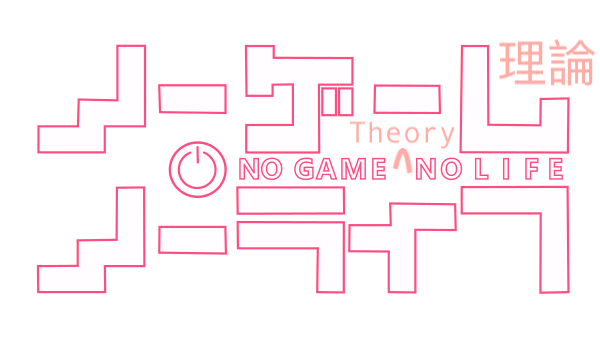
\includegraphics[scale=0.40]{no_game_theory_no_life}
  \caption{No Game (Theory) No Life \cite{ngnl}}
\end{figure}

\section{Introduction}

Contrary to its name, game theory has deep implications beyond playing
games very well - life itself can be thought of as a difficult game.

A connection between game theory and cutting edge machine learning exists
under a mathematical intrepretation of Generative Adversarial Networks (GANs)
- many papers describe GANs as playing a minimax game and converging to a Nash equilibrium.
A machine learning club lecture was written on this topic \cite{thistlethwaite}.
Another connection exists when considering Reinforcement Learning (RL) as
commonly applied to game-playing (exemplified by Google DeepMind's recent
Go, Shogi, and Chess RL system called AlphaZero \cite{DBLP:journals/corr/abs-1712-01815}).
RL, however, is a more general technique that has often been applied
to robotics (see OpenAI's robot hand that solves a Rubik's cube \cite{2019arXiv191007113O}).
Notably, GANs, RL,
and energy based models (EBMs) are all mathematically equivalent (under certain conditions)
\cite{DBLP:journals/corr/FinnCAL16} which gives a nontrivial reason to study game theory -
it advances the cutting edge of machine learning as advances in playing games
directly leads to advancements in GANs, RL, and EBMs.

\section{Algorithms}
\subsection{Minimax}

Minimax is a perfect information game (i.e., a game without hidden states) player.
It views a game as a tree of states, with actions being state transitions (edges in the tree)
and attempts to pick the best subtree at each node.
It does this via a depth-first search: one move away from an end game state,
the best move is obvious - the move that maximizes the immediate utility.
Two moves away, it has the score of all its children, and just pick the best moves from those.
Move up the tree and it can reconstruct the optimal move for each state.

However it's infeasible to actually compute the entire game tree for a nontrivial game.
Therefore, we need to use a heuristic which caps the search depth to something
that is reasonable and is usually human designed (see the Othello project in AI).

One such approach to creating a good Othello player is documented in the Logisthello
bot \cite{Buro97experimentswith}. He essentially assumed the heuristic
was a linear function of features he hand-defined, and solved linear equations
for an optimal heuristic iteratively with backpropagation
(neural networks weren't as popular in the 90's).
The ideal heuristic is obviously the actual utility function - whether one wins or
loses from a given position given optimal play, and having to select features
by hand is time consuming, requires a in-depth knowledge of the given domain,
and may not be optimal. One might consider training a neural network to estimate
the true utility function but there is a paradox -
where does one get the training data for optimal play when one doesn't know
how to play optimally? Logisthello used human Othello games but obviously
that may not be optimal. This paradox is usually resolved through self-play,
where the machine gets iteratively better as more games are played.

\subsection{Monte Carlo Tree Search}

Monte Carlo Tree Search (MCTS) is an algorithm similar to Minimax in the sense
that both are tree searches. However, MCTS is more in line with the ``self-play''
philosophy - it essentially uses the result of a large number of random games
as heuristic for how good a particular position is.
MCTS was used by the AlphaZero system along with RL.

\section{Counterfactual Regret Minimization}

Both algorithms, however, require perfect information. In real life, however, we rarely have perfect information -
one is often uncertain excactly what effect an action can have and other variables.
One such problem is Reconnaissance Blind Chess (RBC), proposed by John Hopkin's
Applied Physics Lab \cite{DBLP:journals/corr/abs-1811-03119}.
RBC is played like regular chess except one does not know
what move their opponent made. Instead, every turn each player can ``sense'' a
3x3 region on the board and learn the positions of every piece in that region.
Minimax, MCTS, and RL do not apply well to such a game.
Thus, the creation of another algorithm is necessary to account for uncertainty.

\subsection{Definitions}

For a perfect information game, playing a game ``optimally'' is well defined
because each state has exactly one ``optimal'' move. However, for a game with
uncertainty, what does it even mean to play optimally?

For simplicity, let us simplify games into \emphasis{normal-form games} \cite{Neller2013AnIT}.
A normal-form game is game with \( N \), the set of \( n \) players,
\( S_i \), the \emphasis{actions} for a player \( i \), \( A \), the set
containing all possible combinations of actions for each player,
and \( u \), the vector giving \emphasis{utilities} (the rewards) for each player
(a particular player's utility is \( u_i \)). These games are commonly represented
by tables, where the row player is player 0 and the column player is player 1.
An entry in the table is pair of numbers in the form \( (u_0, u_1) \),
representing the utility for player 0 and player 1.

\begin{table}[h!]
\begin{center}
\begin{tabular}{ c|c|c|c| }
 \multicolumn{4}{ c }{\begin{tabular}{c c c c c c} & R & & P & & S \end{tabular}} \\
 % & R & P & S \\
 \cline{2-4}
 R & 0, 0 & -1, 1 & 1, -1 \\
 P & 1, -1 & 0, 0 & -1, 1 \\
 S & -1, 1 & 1, -1 & 0, 0 \\
 \cline{2-4}
\end{tabular}
\end{center}
\caption{The payoff table for rock paper scissors}
\end{table}

A game is \emphasis{zero-sum} if each entry adds up to 0.
Finally, a \emphasis{strategy} for a game is a function representing the probablity
that an action is chosen. We notate strategies as \( \sigma_i (s) \), representing
the probability for player \( i \) to use action \( s \in S_i \). \( -i \) refers
to the opponent, so in the case of two players \( S_{-i} = S_{1 - i} \).

Since games under uncertainty are played in a probabilistic manner,
playing the same strategies against each other multiple times will have different results.
Rather than track simple win/losses for a single game, we instead define the
\emphasis{expected utility}, the amount of utility that the player expects to get
per game over the long term.
 The definition of expected value is sum of each value times the probability of that value occuring.
 To use this definition in our game, we sum over each possible value (each entry in the table)
 and the probability that such a value occurs takes into account both player's strategies.

 \[ u_i (\sigma_i, \sigma_{-i}) = \sum_{s \in S_i} \sum_{s' \in S_{-i}} \sigma_i(s) \sigma_{-i} (s') u_i(s, s') \]

Under this framework, we finally arrive at the defintion of optimal play for uncertain games.
A \emphasis{best response} strategy is one that maximizes a player's expected
utility, given the strategies of the opponent(s). If both players play
best responses, the combination of strategies is the \emphasis{Nash equilibrium}.
As we shall see, one intrepretation of the Nash equilibrium is that players cannot
change strategies to gain an advantage - any change in strategy will
yield the same expected utility (this is consistent with the definition of ``maximizing'' because,
intuitively, any movement yields the same function value, so our current position must be a local extrema).
A player is \emphasis{indifferent} if all actions have the same utility.
If both players are indifferent, than that is a Nash equilibrium.

\subsection{Examples}
\subsubsection{Rock Paper Scissors (RPS)}

It seems obvious that the optimal strategy for RPS is to play
rock with \( \frac{1}{3} \) probability, and the same for paper and scissors.
Suppose that one deviated from the optimal strategy and played
\( \frac{1}{2} \) rock, \( \frac{1}{4} \) scissors, and \( \frac{1}{4} \) paper.
What would the optimal response be?
Basic analysis shows that it would be to punish the over-emphasis on rock as much as possible,
by always playing paper (a strategy always playing a single action is known as a
\emphasis{pure strategy}, and a non-pure strategy is a \emphasis{mixed strategy}).
The strategy of always playing paper yields an expected value of
\( \frac{1}{2} (1) + \frac{1}{4} (-1) + \frac{1}{2} (0) = \frac{1}{4} \).
Since playing any action with greater than \( \frac{1}{3} \) leads to a pure strategy
punishing that deviation, the optimal strategy must be the one stated above.

We can also reason why the the solution fulfills our definition of the Nash equilibrium.
Computing the expected values for playing rock, paper, and scissors:
\begin{align*}
u_R = \frac{1}{3} (0) + \frac{1}{3} (-1) + \frac{1}{3} (1) = 0 \\
u_P = \frac{1}{3} (1) + \frac{1}{3} (0) + \frac{1}{3} (-1) = 0 \\
u_S = \frac{1}{3} (-1) + \frac{1}{3} (1) + \frac{1}{3} (0) = 0
\end{align*}

Since the expected value for playing any action is the same, we are indifferent, and
so it must be the Nash equilibrium.

\subsubsection{Pure Strategies}

We saw in RPS that a deviation from the Nash equilibrium led to a pure strategy
being optimal to take advantage of that deviation. Is that generally true?
The answer is yes, and to prove it requires a basic understanding on linear programming.
In normal-form games, our expected utility must be a linear function of
the probabilities. The constraint on the probabilities is that they sum to one
and that each probability is greater or equal to 0.
Given a linear objective function we want to maximize and a linear constraint,
linear programming states that the optimal value occurs at a vertex of the simplex,
or the region of feasible values for each parameter.
Since the constraint \( x_1 + x_2 + \dots + x_n = 1 \) along with \( x_i \geq 0 \)
has a feasible region which is the hyperplane's intersection with each axis,
the vertex of the simplex must be when one probability is 1 and the rest are 0,
fulfilling the definition of a pure strategy.

\subsubsection{A Variant of RPS}

To see one way to compute the Nash equilibrium for normal-form games,
one needs to have a less obviously solved game. Consider RPS, but one
player is handicapped in the sense that they are at a disadvantage if they play
scissors. All interactions are identical to standard RPS
except when player 1 plays scissors:
player one scissors loses against player two scissors,
ties against player two paper, and loses against player two rock.

\begin{figure}[h!]
  \centering
  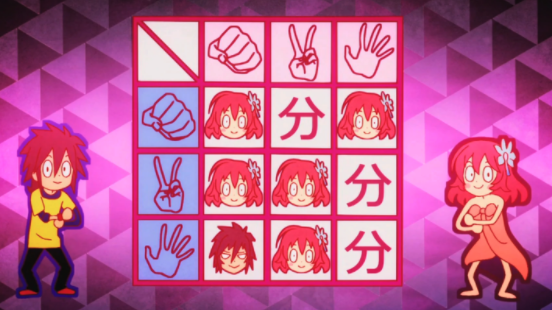
\includegraphics[scale=0.42]{rps_table}
  \caption{Utility table for the game (from \textit{No Game No Life} episode 2, circa 5 minutes)}
\end{figure}

Let us calculate the best response strategy for Stephanie, the girl on the right.
Let player 0 be Sora, the boy on the left, and player 1 be Stephanie.
Let \( p_1 = \sigma_1 (R) \), \( p_2 = \sigma_1 (S) \), and \( p_3 = \sigma_1 (P) \)
(encapsulating Stephanie's strategy).
We have:
\begin{gather}
u_R = p_1 (-1) + p_2 (0) + p_3(-1) = -p_1 - p_3 \\
u_S = p_1 (-1) + p_2 (-1) + p_3(0) = -p_1 - p_2 \\
u_P = p_1 (1) + p_2 (-1) + p_3(0)  =  p_1 - p_2 \\
p_1 + p_2 + p_3 = 1
\end{gather}

Let \( u_R = u_S = u_P \), giving us three equations and set (2) equal to (3):
\begin{align*}
-p_1 - p_2 &= p_1 - p_2 \\
p_1 &= 0
\end{align*}

Set (1) equal to (2):
\begin{align*}
-p_1 - p_3 &= -p_1 - p_2 \\
p_2 &= p_3
\end{align*}

Because of (4), \( p_2 = \frac{1}{2} \) and \( p_3 = \frac{1}{2} \).
Thus, the optimal strategy for Stephanie is to never play rock and flip a coin
between scissors and paper. Doing similar logic for Sora, his optimal strategy
is to play \( \begin{bmatrix} \frac{1}{2} & \frac{1}{4} & \frac{1}{4} \end{bmatrix} \).
Using the expected value formula from earlier, Stephanie's expected value is
\( \frac{1}{2} \) and since this is a zero-sum game, Sora's is \( -\frac{1}{2} \).

\begin{figure}[h!]
  \centering
  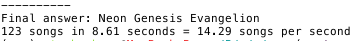
\includegraphics[scale=0.2]{result}
  \caption{The end result of the game, which is consistent with our calculations.}
\end{figure}

\subsection{Regret}

Normal-form games can be solved as a linear system of equations as shown above.
However, for games that are not normal-form, a more general algorithm is necessary
to calculate the Nash equilibrium.
One such algorithm is based off the concept of regret.

Suppose we are playing (standard) RPS and we played rock while our opponent played paper.
We regret not playing paper and drawing, but we regret not playing scissors, and winning, even more.
\emphasis{Regret} of an action is formally defined as the difference
between the utility of that action and the action we originally chose.
Given this definition, we regretted not playing paper 1 (\( 0 - (-1) \)) and
not playing scissors 2 (\( 1 - (-1) \)).
In order to use regret to find the Nash equilibrium, one obvious goal
is to minimize regret.
However, simply picking the action we regret most at a point in time
is ineffective as our opponent can track our regrets and predict our actions.
Instead, we use \emphasis{regret matching},
or creating a strategy where the probability of playing an action
is proportional to the amount we regret not playing it.
In order to turn our regrets into probabilities, take the sum of all the positive regrets
(if the regrets are negative, we will never play those actions).
Then, the probability of playing a given action is the amount we regret it divided by the total regret.
However, even regret matching doesn't guarentee convergence to the Nash equilibrium.
Instead, the \emphasis{average} of the strategies generated by regret matching
converges to the Nash equilibrium as the number of trials approaches infinity.
The algorithm is as follows:

\begin{itemize}
  \item Initialize regrets to 0
  \item For some number of iterations:
  \begin{itemize}
    \item Compute a strategy with regret-matching
    \item Add the strategy to the cumulative strategy sum
    \item Select actions based off the strategy
    \item Compute regrets
    \item Add the regrets to the cumulative regrets
  \end{itemize}
  \item Return the average strategy, the strategy sum divided by the number of iterations
\end{itemize}

It is not obvious how this algorithm generalizes to non normal-games,
but it basically becomes a tree search similar to minimax.
The resulting algorithm is called counterfactual regret minimization (CFR) and
is extremely general and can be applied to non normal-games,
like Poker and RBC.

However, CFR has the same problems as minimax, namely the tree size growing
exponentially, making a full traversal impractical. One way to resolve this
is to use Monte Carlo methods, in a similar way to MCTS \cite{DBLP:conf/nips/GibsonBLS12}, creating Monte Carlo CFR (MCCFR).
Instead of searching through every possible action, one can randomly sample a
subset of the possible actions.
Another way to resolve this
is to use a heuristic, but in this case the ``heuristic'' is known as an
\emphasis{abstraction}. An abstraction is a simplification of the original
game, losing information as a trade off for time.
Abstractions are commonly used in Poker, one example would be treating
a bet of 90 chips as the same as a bet of 100 chips.

The same problems with heuristics apply to abstractions. CFR applied to Poker
often relies on hand-crafted, domain-specific, and ad-hoc abstractions.
Machine learning provides a solution however, by using deep neural networks (NNs)
on CFR.

\subsection{Deep CFR}

The idea of Deep CFR is to use a NN to approximate the results CFR would have
produced without abstractions \cite{DBLP:journals/corr/abs-1811-00164}.
In particular, they use MCCFR to sample states and train one NN (called the ``value'' network) on the regrets produced by MCCFR.
They also train another network, called the ``policy'' network,
which approximates the average strategy, the thing that converges
to the Nash equilibrium.

\subsection{Single Deep CFR}

An optimization on Deep CFR is Single Deep CFR, or a variant which
only uses a single value network, discarding the policy network \cite{DBLP:journals/corr/abs-1901-07621}. They accomplish this by storing all iteration strategies,
increasing the memory usage but reducing prediction error and removing the need
for the policy network to predict the average strategy.

\subsection{Neural Fictitious Self-Play (NFSP)}

A competitor to Deep CFR is NFSP, which relies on the concept of fictitious
self-play instead of regret minimization, and uses RL as deep learning \cite{DBLP:journals/corr/HeinrichS16}.
Fictitious self-play is less well documented than CFR, however.

\section{Conclusion}

Game theory is becoming increasingly relevant as machine learning
becomes more and more popular. Traditional game-playing algorithms
like minimax, MCTS, and RL struggle on imperfect information games,
thus algorithms like CFR and NFSP are the next step
in game theory. Machine learning techniques can be applied to
CFR in order to remove the human-designed elements common
to most game-playing algorithms.

\newpage
\printbibliography
\end{document}
